\documentclass[10pt,a4paper]{article}
\usepackage{amsmath}
\usepackage{amssymb}
\usepackage{graphicx}
\usepackage{color}
\usepackage{fancyhdr}
\usepackage{fancyvrb}
\usepackage[margin=3.5cm]{geometry}
\usepackage{framed}
\usepackage{enumerate}
\usepackage{textcomp}
\def\ket#1{\left|#1\right\rangle}
\def\bra#1{\left\langle#1\right|}
\def\braket#1{\left\langle#1\right\rangle}

\definecolor{linkcol}{rgb}{0.0, 0.0, 0.7}
\usepackage[colorlinks=true,urlcolor=linkcol,citecolor=black,linkcolor=linkcol]{hyperref}

\setcounter{section}{1}
\renewcommand\thesection{\arabic{section}}
\renewcommand\thesubsection{\thesection.\arabic{subsection}}

\fancyhf{}
\lhead{\tiny Y.~D.~Chong (2020)}
\rhead{\scriptsize MH2801: Complex Methods for the Sciences}
\lfoot{}
\rfoot{\thepage}
\pagestyle{fancy}

\begin{document}
\setcounter{page}{14}

\section{Integrals}
\label{integrals}

If we have a function $f(x)$ which is well-defined for some $a \le x
\le b$, its integral over those two values is defined as
\begin{equation}
  \int_a^b dx\; f(x) \;=\; \lim_{N \rightarrow 0} \, \sum_{n=0}^{N} \Delta x\; f(x_n) \;\;\;\mathrm{where}\;\; x_n = a + n\Delta x, \;\; \Delta x \equiv \left(\frac{b-a}{N}\right).
\end{equation}
This is called a \textbf{definite integral}, and represents the area
under the graph of $f(x)$ in the region between $x=a$ and $x=b$,
as shown in the figure below. The function $f(x)$ is called the
\textbf{integrand}, and the two points $a$ and $b$ are called the
\textbf{bounds} of the integral. The interval between the two bounds is
divided into $N$ segments, of length $(b-a)/N$ each. Each term in
the sum represents the area of a rectangle, and as
$N\rightarrow \infty$, the sum converges to the area under the curve.

\begin{figure}[h]
  \centering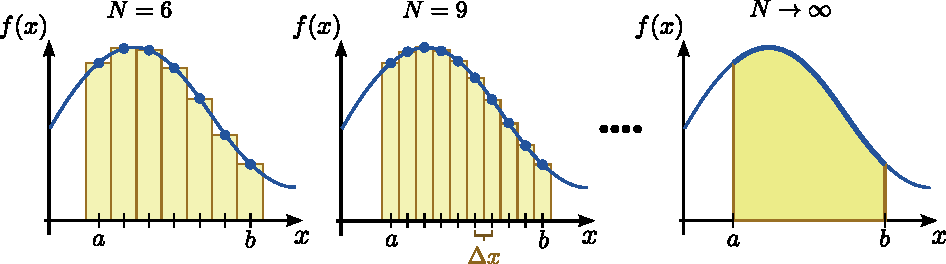
\includegraphics[width=0.9\textwidth]{definite_integral}
\end{figure}

A \textbf{multiple integral} involves integration over more than one
variable. For instance, when we have a function $f(x_1,x_2)$ that
depends on two independent variables, $x_1$ and $x_2$, we can
perform a double integral by integrating over one variable first, then
the other variable:
\begin{equation}
\int_{a_1}^{b_1} dx_1 \int_{a_2}^{b_2} dx_2 \; f(x_1, x_2) \equiv \int_{a_1}^{b_1} dx_1 F(x_1)\quad\text{where}\;\;F(x_1) \equiv \int_{a_2}^{b_2} dx_2 \; f(x_1, x_2).
\end{equation}


\subsection{Basic properties of definite integrals}
\label{basic-properties-of-definite-integrals}

The value of a definite integral depends only on the integrand, and the
two integration bounds. The variable which is integrated over is a
\textbf{dummy variable}, which means that changing the symbol does not
affect the value of the overall expression:
\begin{equation}
\int_a^b dx\; f(x) = \int_a^b dy\; f(y).
\end{equation}
Since the value of the integral does not depend on the dummy variable,
it is nonsensical to write something like
\begin{equation*}
\frac{d}{dx}\; \left[\int_a^b dx\; f(x)\right]. \;\;\;(\text{Nonsense expression}!)
\end{equation*}

Since an integral is defined as the limiting form of a sum, it can be
algebraically manipulated in the same way as a summation expression. For
instance, an integral of a linear combination is equal to a linear
combination of two integrals \emph{with the same bounds}:
\begin{equation}
\int_a^b dx \;\Big[c_1 \,f_1(x) + c_2\, f_2(x)\Big] = c_1 \int_{a}^{b} dx \; f_1(x)\;\, +\;\, c_2 \int_{a}^{b} dx\; f_2(x).
\end{equation}
This is analogous to how the summation of a linear combination is equal
to the linear combination of separate summations:
\begin{equation}
\sum_{n = p}^{q} \Big[ c_1  A_n \, + \, c_2 B_n\Big] = c_1 \sum_{n = p}^{q} A_n \, + \, c_2 \sum_{n = p}^{q} B_n.
\end{equation}
For a similar reason, multiple integrals can be manipulated like
multiple summations. If we have a double integral where the integrals
have \emph{independent} bounds, we can swap the order of the integrals:
\begin{equation}
  \int_{a_1}^{b_1} dx_1 \int_{a_2}^{b_2} dx_2 \;\; f(x_1, x_2)
  = \int_{a_2}^{b_2} dx_2 \int_{a_1}^{b_1} dx_1 \;\; f(x_1, x_2).
\end{equation}
This is analogous to how we can swap the order of two independent
summations. Note, however, that this manipulation is invalid if the
integration bounds are not independent. For instance, if the upper or
lower bound of the inner integral depends on the integration variable of
the outer integral, we can't swap the two integrals:
\begin{equation*}
\int_{a_1}^{b_1} dx_1 \int_{a_1}^{x_1} dx_2 \;\; f(x_1, x_2) \ne \int_{a_1}^{x_1} dx_2 \int_{a_1}^{b_1} dx_1 \;\; f(x_1, x_2).\;\; (\text{Nonsense expression}!)
\end{equation*}
(Note that the expression on the right is nonsensical: $x_1$ is meant
to be a dummy variable, yet it exists outside of any integration sign.)

\subsection{Integrals as antiderivatives}
\label{integrals-as-antiderivatives}

Since the value of a definite integral depends on the values of the
upper and lower bounds, we can ask what happens to the value of the
definite integral when either bound is varied. Using the defintion of
the derivative from the previous chapter, we can show that
\begin{align}
  \frac{d}{db} \left[\int_a^b dx\; f(x)\right] &= f(b), \\
  \frac{d}{da} \left[\int_a^b dx\; f(x)\right] &= -f(a).
\end{align}
To prove the first equation, observe that increasing the upper bound
from $b$ to $b + \delta b$ increases the area under the curve by $f(b)
\delta b$ (to lowest order in $\delta b$). Hence, the definite
integral's rate of change with $b$ is $f(b)$. Likewise, increasing the
lower bound from $a$ to $\delta a$ \emph{decreases} the area under the
curve, leading to a rate of change of $-f(a)$.

From the above result, we define the concept of an \textbf{indefinite
integral}, or \textbf{antiderivative}, as the inverse of a derivative
operation:
\begin{equation}
\int^x dx' f(x') \equiv F(x) \;\;\mathrm{such}\;\mathrm{that}\;\; \frac{d}{dx}F(x) = f(x).
\end{equation}
Since derivatives are not one-to-one (i.e., two different functions can
have the same derivative), an antiderivative does not have a unique,
well-specified value. Rather, its value is only defined up to an
additive constant, called an \textbf{integration constant}. A definite
integral, by contrast, always has a well-defined value.

Finding antiderivatives is much harder than differentiation. Once you
know how to differentiate a few special functions, differentiating
some combination of those functions usually involves a straightforward
(if tedious) application of composition rules. By contrast, there is
no general systematic procedure for symbolic integration. Integration
often requires creative steps, like guessing a solution and checking
if its derivative yields the desired integrand.

Some common techniques are summarized in the following sections;
others will be introduced later in this course.

\subsection{Integration by parts}

If the integrand consists of two factors, and you know the
antiderivative of one of the factors, you can \textbf{integrate by
  parts} by shifting the derivative onto the other factor:
\begin{equation}
\int_a^b dx \; f(x) \, \frac{dg}{dx} \;=\; \Big[\,f(x)\, g(x)\,\Big]_a^b - \int_a^b \frac{df}{dx}\, g(x). 
\end{equation}
The first term on the right hand side is a constant denoting
$[f(a)g(a) - f(b)g(b)]$. Hopefully, the integral in the second term is
easier to solve than the original integral.

Judicious use of integration by parts is a key step for solving many
integrals. For example, consider
\begin{equation}
\int_a^b dx\; x \, e^{\gamma x}.
\end{equation}
The integrand consists of two factors, $x$ and $e^{\gamma x}$; we
happen to know the antiderivative of both factors. Integrating by parts
lets us replace one of these factors with its antiderivative, while
applying an additional derivative on the other factor. The smart thing
to do is to apply the derivative on the $x$ factor, and the
antiderivative on the $e^{\gamma x}$:
\begin{align}
  \int_a^b dx\; x\, e^{\gamma x} \;&=\; \left[\;x\, \frac{e^{\gamma x}}{\gamma}\, \right]_a^b - \int_a^b dx\; \frac{e^{\gamma x}}{\gamma} \\
  &=\; \left[\;x\, \frac{e^{\gamma x}}{\gamma} - \frac{e^{\gamma x}}{\gamma^2} \,\right]_a^b.
\end{align}
Whenever we finish doing an integral, it is good practice to
double-check the result by making sure the dimensions match up. Note
that $\gamma$ has units of inverse $x$, so the integral on the
left-hand side has units of $x^2$. The solution on the right hand side
has two terms, with units $x/\gamma$ and $1/\gamma^2$; both of these
are equivalent to units of $x^2$, which is what we need!

\subsection{Change of variables}
\label{change-of-variables}

Another useful technique for solving integrals is to change variables.
Consider the integral
\begin{equation}
\int_0^\infty \frac{dx}{x^2 + 1}.
\end{equation}
We can solve this by making a change of variables $x = \tan(u)$. This
involves (i) replacing all occurences of $x$ in the integrand with
$\tan(u)$, (ii) replacing the integral limits, and (iii) replacing
$dx$ with $(dx/du) \, du = 1/[\cos(u)]^2 du$:
\begin{align}
  \int_0^\infty \frac{dx}{x^2 + 1} &= \int_0^{\pi/2} \frac{1}{[\tan(u)]^2 + 1} \cdot \frac{1}{[\cos(u)]^2} \; du \\
  &= \int_0^{\pi/2} \frac{1}{[\sin(u)]^2 + [\cos(u)]^2} \; du.
\end{align}
Due to the Pythagorean theorem, the integrand reduces to 1, so
\begin{equation}
\int_0^\infty \frac{dx}{x^2 + 1} = \int_0^{\pi/2} du = \frac{\pi}{2}.
\end{equation}
Clearly, this technique often requires some cleverness and/or
trial-and-error in choosing the right change of variables.

\subsection{The Gaussian integral}
\label{the-gaussian-integral}

Here's a famous integral:
\begin{equation}
\int_{-\infty}^\infty \; e^{-\gamma x^2} \; dx.
\end{equation}
The integrand is called a \textbf{Gaussian}, or \textbf{bell curve},
and is plotted below. The larger the value of $\gamma$, the more
narrowly-peaked the curve.

\begin{figure}[h]
  \centering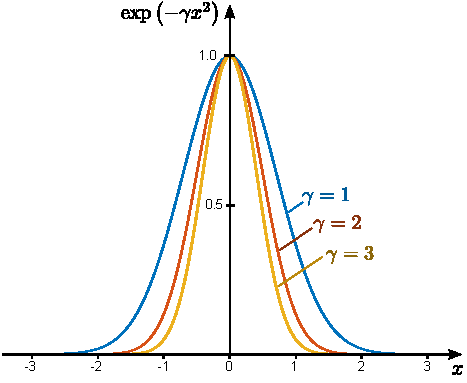
\includegraphics[width=0.6\textwidth]{gaussian}
\end{figure}
    
The integral was solved by
\href{http://en.wikipedia.org/wiki/Carl_Friedrich_Gauss}{Gauss} in a
brilliant way. Let $I(\gamma)$ denote the value of the integral. Then
$I^2$ is just two independent copies of the integral, multiplied
together:
\begin{equation}
I^2(\gamma) = \left[\int_{-\infty}^\infty dx\; e^{-\gamma x^2}\right] \times \left[\int_{-\infty}^\infty dy\; e^{-\gamma y^2}\right].
\end{equation}
Note that in the second copy of the integral, we have changed the
``dummy'' label $x$ (the integration variable) into $y$, to avoid
ambiguity. Now, this becomes a two-dimensional integral, taken over the
entire 2D plane:
\begin{equation}
I^2(\gamma) = \int_{-\infty}^\infty dx\, \int_{-\infty}^\infty dy \; e^{-\gamma (x^2+y^2)}.
\end{equation}
Next, change from Cartesian to polar coordinates:
\begin{equation}
I^2(\gamma) = \int_{0}^\infty dr\, r \int_{0}^{2\pi} d\phi \; e^{-\gamma r^2} = \left[ \int_{0}^\infty dr\, r \, e^{-\gamma r^2}\right] \times \left[\int_{0}^{2\pi} d\phi \right] = \frac{1}{2\gamma} \cdot 2\pi.
\end{equation}
By taking the square root, we arrive at the result
\begin{equation}
I(\gamma) = \int_{-\infty}^\infty dx \; e^{-\gamma x^2} = \sqrt{\frac{\pi}{\gamma}}.
\end{equation}

\subsection{Differentiating under the integral sign}
\label{differentiating-under-the-integral-sign}

In the previous section, we noted that if an integrand contains a
parameter (denoted $\gamma$) which is independent of the integration
variable (denoted $x$), then the definite integral can itself be
regarded as a function of $\gamma$. It can then be shown that taking
the derivative of the definite integral with respect to $\gamma$ is
equivalent to taking the \emph{partial derivative} of the integrand:
\begin{equation}
\frac{d}{d\gamma} \, \left[\int_a^b dx\; f(x,\gamma)\right] = \int_a^b dx \; \frac{\partial f}{\partial \gamma}(x,\gamma).
\end{equation}

This operation, called \textbf{differentiating under the integral sign},
was first used by
\href{https://en.wikipedia.org/wiki/Gottfried_Wilhelm_Leibniz}{Leibniz},
one of the inventors of calculus. It can be applied as a technique for
solving integrals, popularized by
\href{https://en.wikipedia.org/wiki/Richard_Feynman}{Richard Feynman}
in his book
\href{https://en.wikipedia.org/wiki/Surely_You\%27re_Joking,_Mr._Feynman!}{\emph{Surely You're Joking, Mr.~Feynman!}}.

Here is the method.  Given a definite integral $I_0$:
\begin{enumerate}
\item Come up with a way to generalize the integrand, by introducing a
  parameter $\gamma$, such that the generalized integral becomes a
  function $I(\gamma)$ which reduces to the original integral $I_0$
  for a particular parameter value, say $\gamma = \gamma_0$.

\item Differentiate under the integral sign. If you have chosen the
  generalization right, the resulting integral will be easier to
  solve, so...

\item Solve the integral to obtain $I'(\gamma)$.

\item Integrate $I'$ over $\gamma$ to obtain the desired integral
  $I(\gamma)$, and evaluate it at $\gamma_0$ to obtain the desired
  integral $I_0$.
\end{enumerate}

An example is helpful for demonstrating this procedure. Consider the
integral
\begin{equation}
  \int_{0}^\infty dx \; \frac{\sin(x)}{x}.
\end{equation}
First, (i) we generalize the integral as follows (we'll soon see why):
\begin{equation}
  I(\gamma) = \int_{0}^\infty dx \; \frac{\sin(x)}{x}\, e^{-\gamma x}.
\end{equation}
The desired integral is $I(0)$. Next, (ii) differentiating under the
integral gives
\begin{equation}
  I'(\gamma) = - \int_{0}^\infty dx \; \sin(x)\, e^{-\gamma x}.
\end{equation}
Taking the partial derivative of the integrand with respect to
$\gamma$ brought down a factor of $-x$, cancelling out the troublesome
denominator. Now, (iii) we solve the new integral, which can be done
by integrating by parts twice:
\begin{align}
  I'(\gamma) &= \left[\cos(x)\,e^{-\gamma x}\right]_0^\infty + \gamma \int_{0}^\infty dx \; \cos(x)\, e^{-\gamma x} \\
  &= -1 + \gamma \left[\sin(x)\,e^{-\gamma x}\right]_0^\infty + \gamma^2 \int_{0}^\infty dx \; \sin(x)\, e^{-\gamma x} \\
  &= -1 - \gamma^2 I'(\gamma).
\end{align}
Hence,
\begin{equation}
  I'(\gamma) = - \frac{1}{1+\gamma^2}.
\end{equation}
Finally, (iv) we need to integrate this over $\gamma$. But we already
saw how to do this particular integral in
Section~\ref{change-of-variables}, and the result is
\begin{equation}
  I(\gamma) = A - \tan^{-1}(\gamma),
\end{equation}
where $A$ is a constant of integration. When
$\gamma \rightarrow \infty$, the integral must vanish, which implies
that $A = \tan^{-1}(+\infty) = \pi/2$. Finally, we arrive at the
result
\begin{equation}
  \int_{0}^\infty dx \; \frac{\sin(x)}{x} = I(0) = \frac{\pi}{2}.
\end{equation}
When we discuss contour integration in Chapter 8, we will see a more
straightforward way to do this integral.

\subsection{Exercises}
\label{exercises}

\begin{enumerate}
\item
  Consider the step function
  \begin{equation}
    \Theta(x) = \left\{\begin{array}{ll} 1, &\;\;\;\textrm{for} \; x \ge 0\\ 0,&\;\;\; \textrm{otherwise.}\end{array}\right.
  \end{equation}
  Write down an expression for the antiderivative of $\Theta(x)$, and
  sketch its graph.

\item
  Show that
  \begin{equation}
    \int_0^{2\pi} dx\, [\sin(x)]^2 = \int_0^{2\pi} dx\, [\cos(x)]^2 = \pi.
  \end{equation}

\item
  Calculate the following definite integrals:

  \begin{enumerate}[(a)]
  \item $\displaystyle\int_{0}^\pi dx\; x^2 \sin(2x)$
  \item $\displaystyle\int_{1}^\alpha dx\; x \ln(x)$
  \item $\displaystyle\int_0^\infty dx\;e^{-\gamma x} \, \cos(x)$
  \item $\displaystyle\int_0^\infty dx\;e^{-\gamma x} \, x \cos(x)$
  \item $\displaystyle\int_{-\infty}^\infty dx\;e^{-\gamma |x|}$
  \item $\displaystyle \int_{-\infty}^\infty dx \;e^{-|x+1|} \sin(x)$
  \end{enumerate}

\item
  By differentiating under the integral, solve
  \begin{equation}
    \int_0^1 dx\; \frac{x^2-1}{\ln(x)}.
  \end{equation}
  Hint: replace $x^2$ in the numerator with $x^\gamma$.
  \hfill{\scriptsize [solution~available]}

\item
  Let $f(x,y)$ be a function that depends on two inputs $x$ and
  $y$, and define
  \begin{equation}
    I(x) = \int_0^x f(x,y) dy.
  \end{equation}
  Prove that
  \begin{equation}
    \frac{dI}{dx} = f(x,y) + \int_0^x \frac{\partial f}{\partial x}(x,y) \;dy.
  \end{equation}

\item
  Consider the ordinary differential equation
  \begin{equation}
    \frac{dy}{dt} = - \gamma y(t) + f(t),
  \end{equation}
  where $\gamma > 0$ and $f(t)$ is some function of $t$. The solution
  can be written in the form
  \begin{equation}
    y(t) = y(0) + \int_0^t dt' \, e^{-\gamma(t-t')} \, g(t').
  \end{equation}
  Find the appropriate function $g$, in terms of $f$ and $y(0)$.
  \hfill{\scriptsize [solution~available]}
\end{enumerate}

\end{document}
